\documentclass[a4paper,12pt]{article}

\author{}
\title{\\
\large \\
\small }
\date{January 14, 2022}

\usepackage[utf8]{inputenc}
\usepackage{graphicx}
\usepackage{float}
\usepackage[T1]{fontenc}
\usepackage{textcomp}
\usepackage{amsmath, amssymb}

\begin{document}
% \maketitle

  \begin{titlepage}
    % \drop=0.1\textheight
    \centering
    \vspace*{\baselineskip}
    \rule{\textwidth}{1.6pt}\vspace*{-\baselineskip}\vspace*{2pt}
    \rule{\textwidth}{0.4pt}\\[\baselineskip]
    {\LARGE Density Calculation in the \\[0.1\baselineskip]
        Smoothed-Particle Hydrodynamics \\[0.3\baselineskip]
    Method using Parallel Programming}\\[0.2\baselineskip]
  
    \rule{\textwidth}{0.4pt}\vspace*{-\baselineskip}\vspace{3.2pt}
    \rule{\textwidth}{1.6pt}\\[\baselineskip]
    \scshape
    Supercomputing Modelling Final Exam Project\\
    \par
    January 14, 2022\\
    \vspace*{2\baselineskip}
    % Edited by \\[\baselineskip]
    {\Large  Sof\'ia Bel\'en L\'opez Vicens\par}
    \vspace*{2\baselineskip}
    % {\itshape Moscow Institute of Physics and Technology\par}

    \vfill
    
\includegraphics[width=0.4\textwidth]{img/mipt.jpg}
    % {\scshape year} \\
    % {\large THE PUBLISHER}\par
  \end{titlepage}

\newpage
\section{Density Heat Maps}

\begin{figure}[H]
    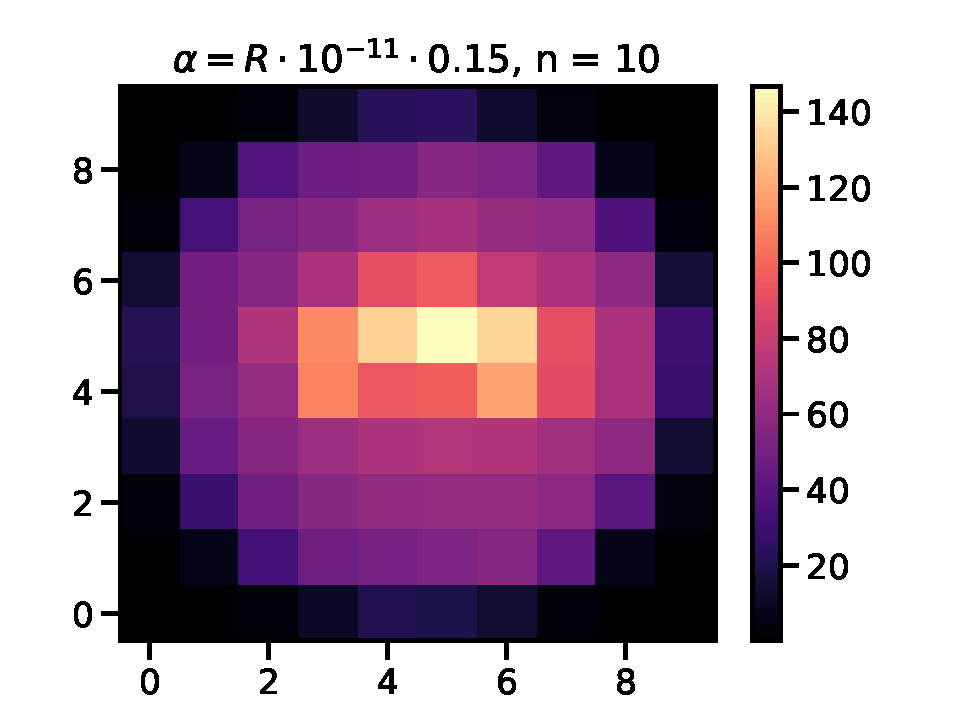
\includegraphics[width=.6\textwidth]{../img-mpi/graph10-0.pdf}\hfill
    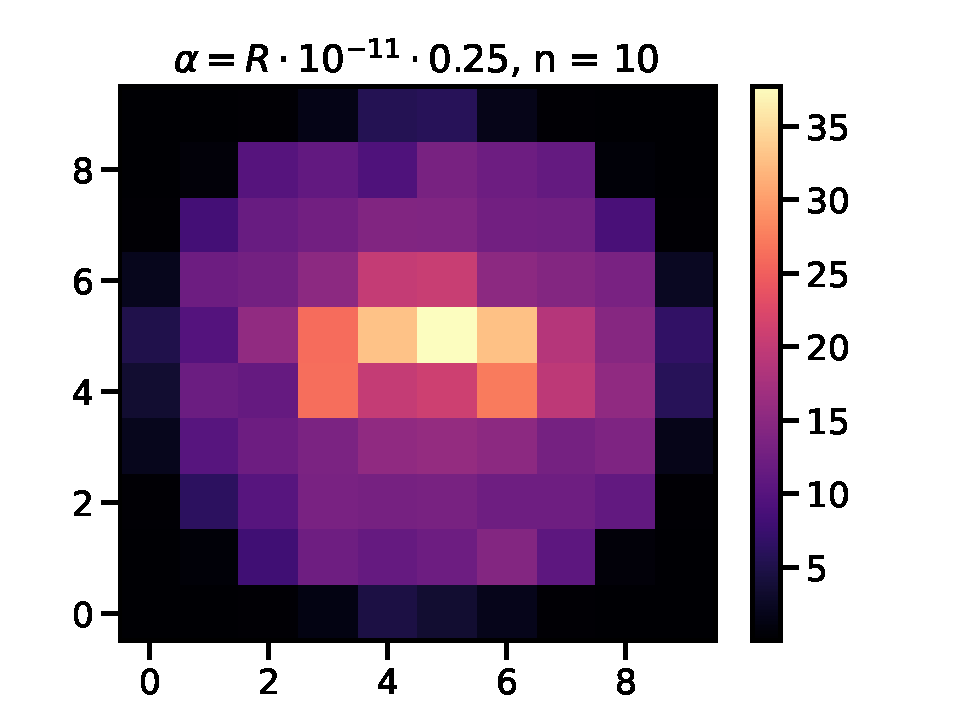
\includegraphics[width=.6\textwidth]{../img-mpi/graph10-1.pdf}\hfill
    \\[\smallskipamount]
    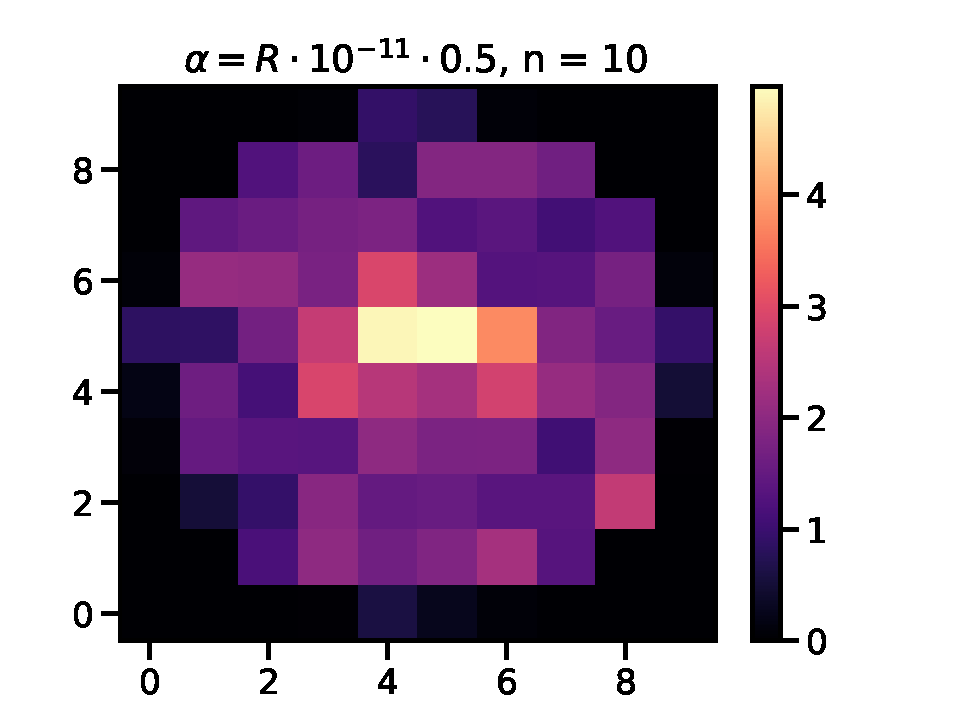
\includegraphics[width=.6\textwidth]{../img-mpi/graph10-2.pdf}\hfill
    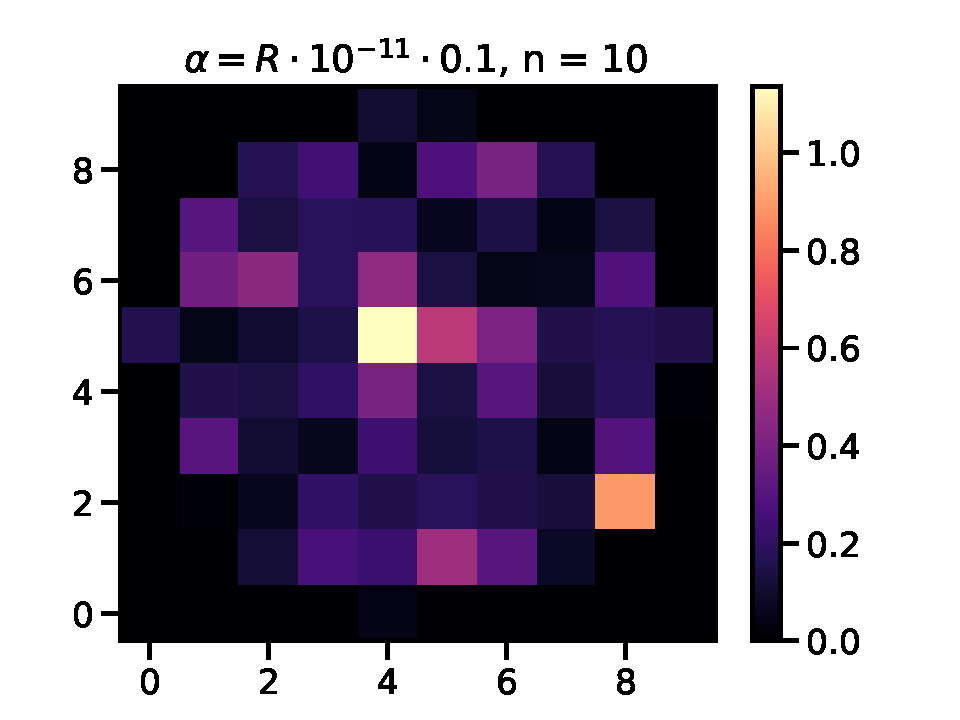
\includegraphics[width=.6\textwidth]{../img-mpi/graph10-3.pdf}
    \caption{Comparison of the effect of the parameter \(\alpha\)
    for \(n_x = n_z = 10\).}
\end{figure}

\begin{figure}[H]
    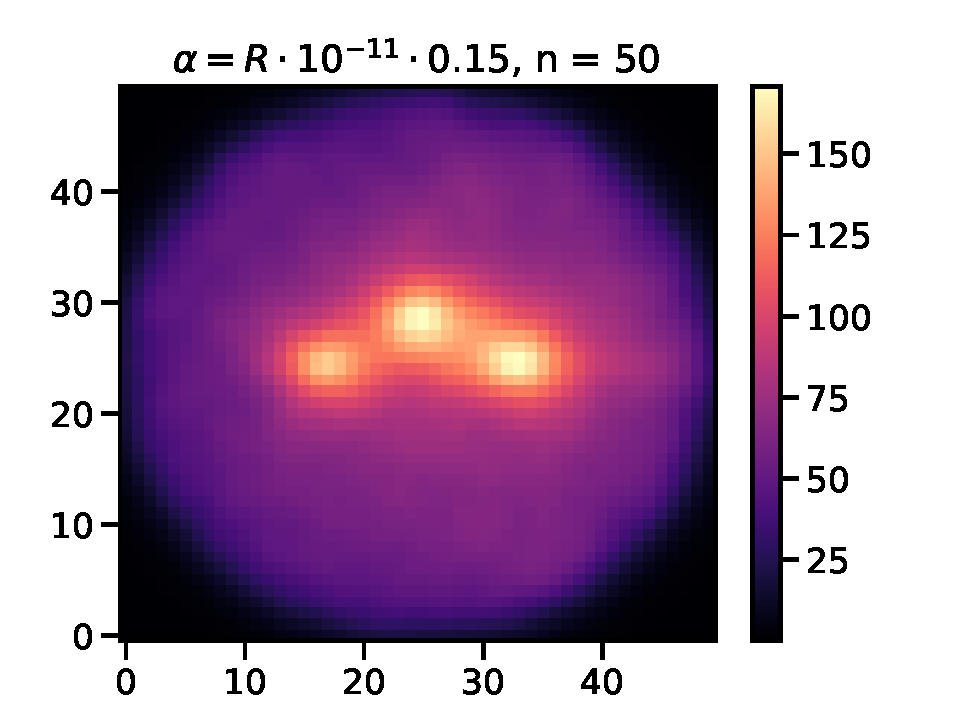
\includegraphics[width=.6\textwidth]{../img-mpi/graph50-0.pdf}\hfill
    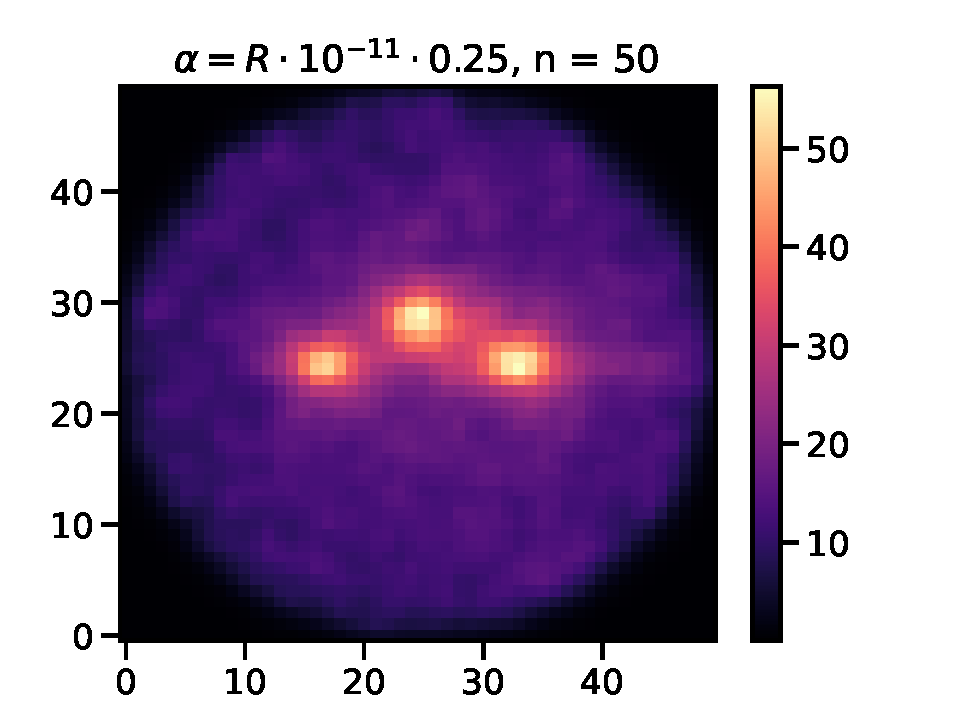
\includegraphics[width=.6\textwidth]{../img-mpi/graph50-1.pdf}\hfill
    \\[\smallskipamount]
    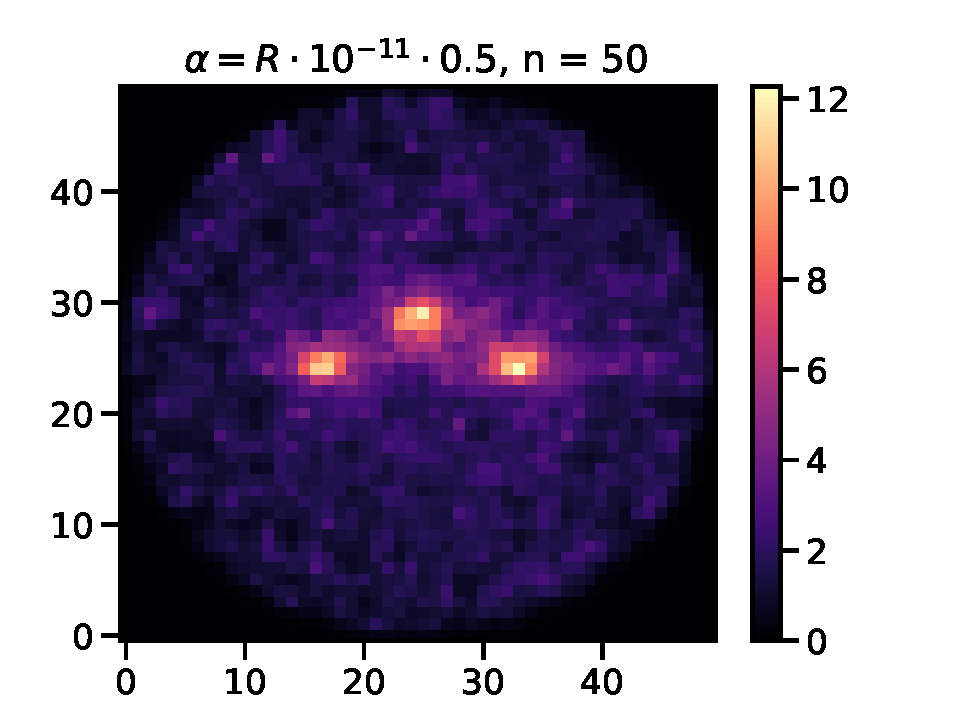
\includegraphics[width=.6\textwidth]{../img-mpi/graph50-2.pdf}\hfill
    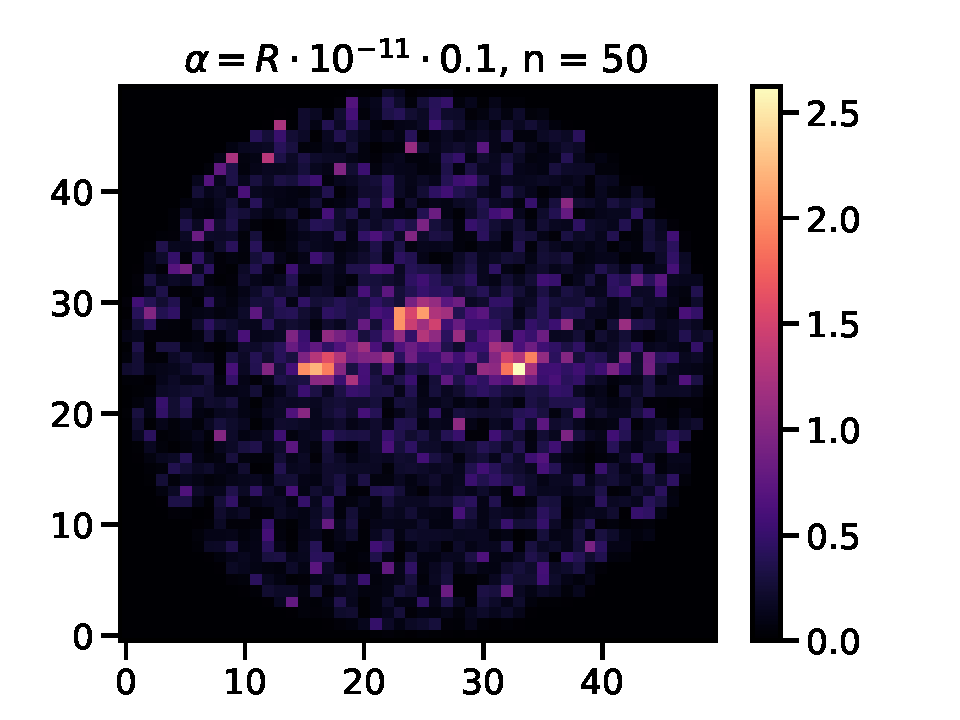
\includegraphics[width=.6\textwidth]{../img-mpi/graph50-3.pdf}
    \caption{Comparison of the effect of the parameter \(\alpha\)
    for \(n_x = n_z = 50\).}
\end{figure}

\begin{figure}[H]
    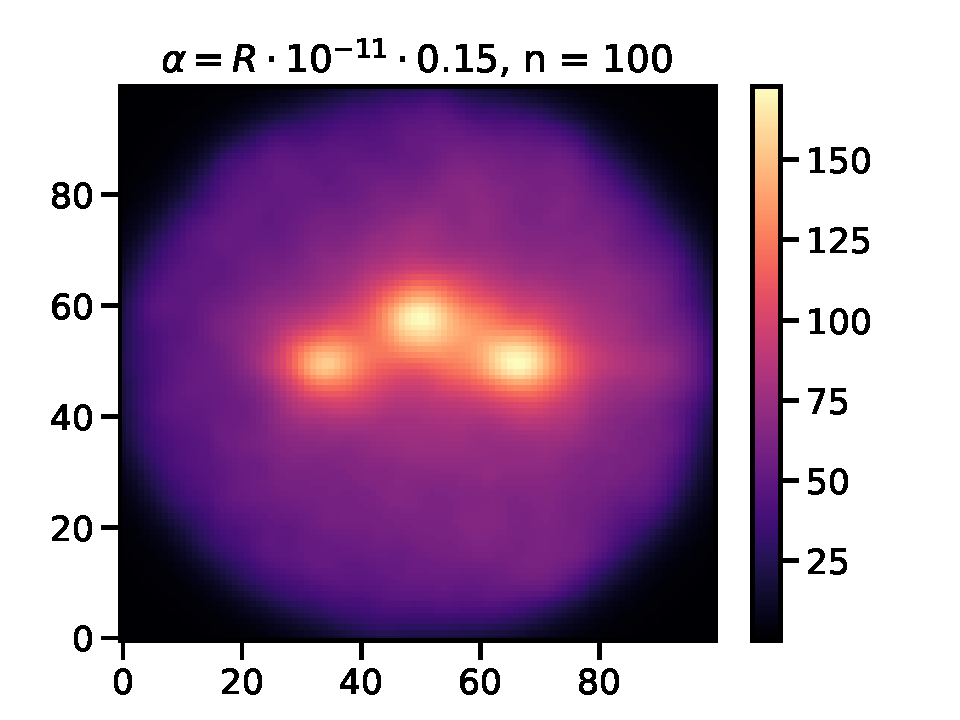
\includegraphics[width=.6\textwidth]{../img-mpi/graph100-0.pdf}\hfill
    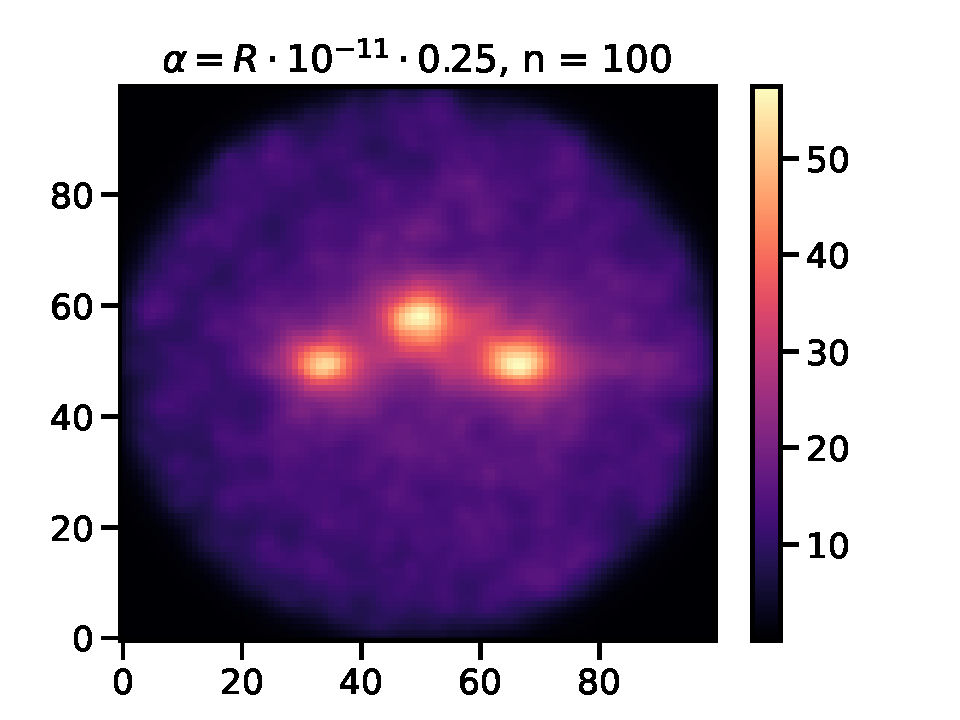
\includegraphics[width=.6\textwidth]{../img-mpi/graph100-1.pdf}\hfill
    \\[\smallskipamount]
    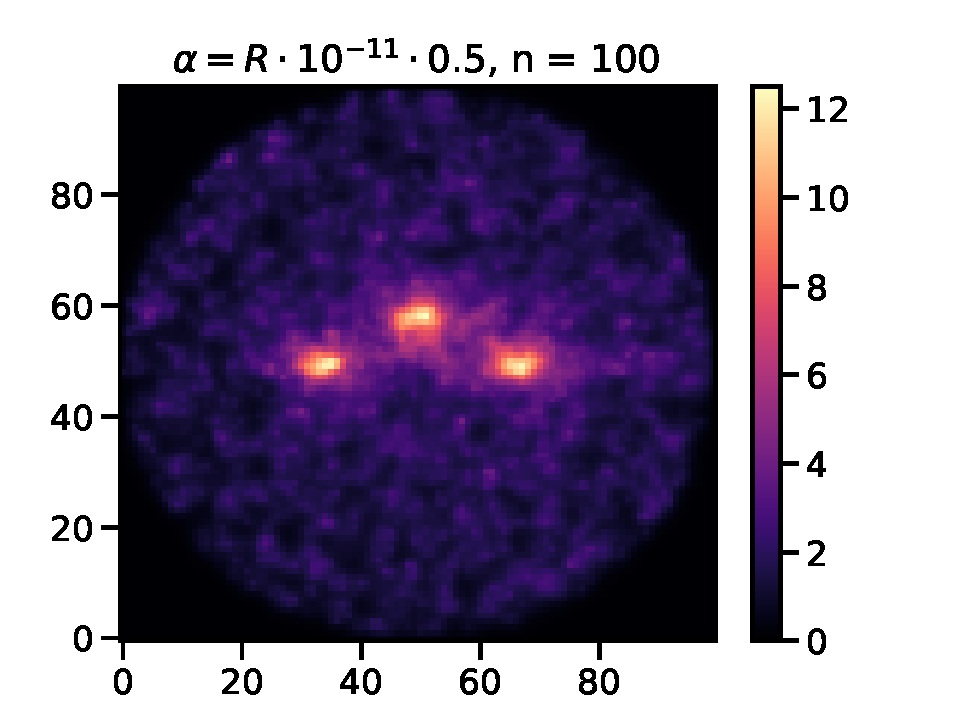
\includegraphics[width=.6\textwidth]{../img-mpi/graph100-2.pdf}\hfill
    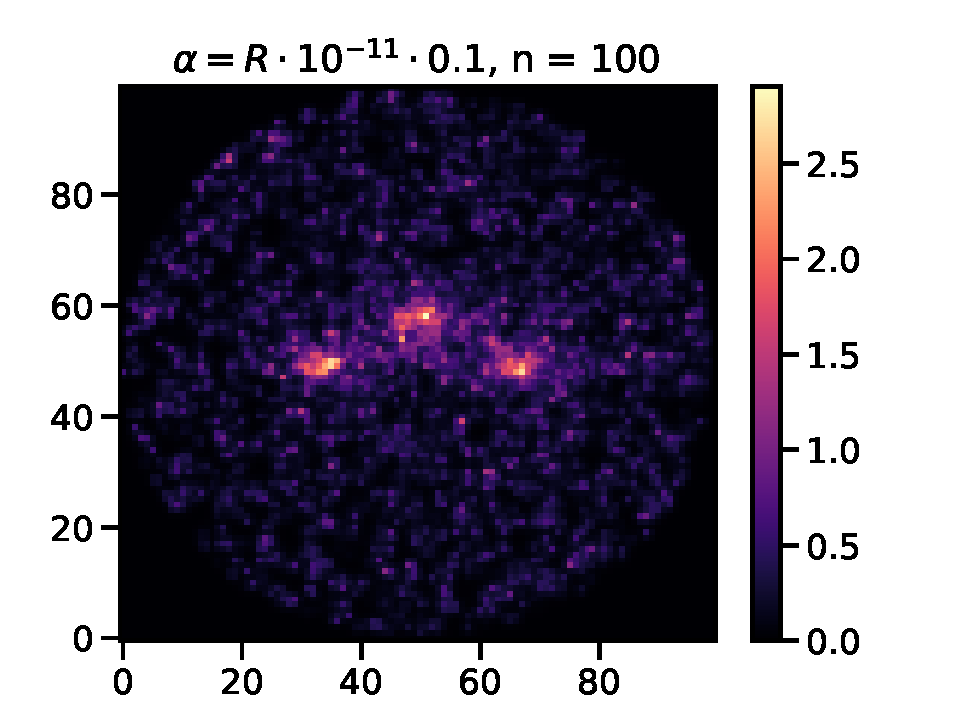
\includegraphics[width=.6\textwidth]{../img-mpi/graph100-3.pdf}
    \caption{Comparison of the effect of the parameter \(\alpha\)
    for \(n_x = n_z = 100\).}
\end{figure}

\begin{figure}[H]
    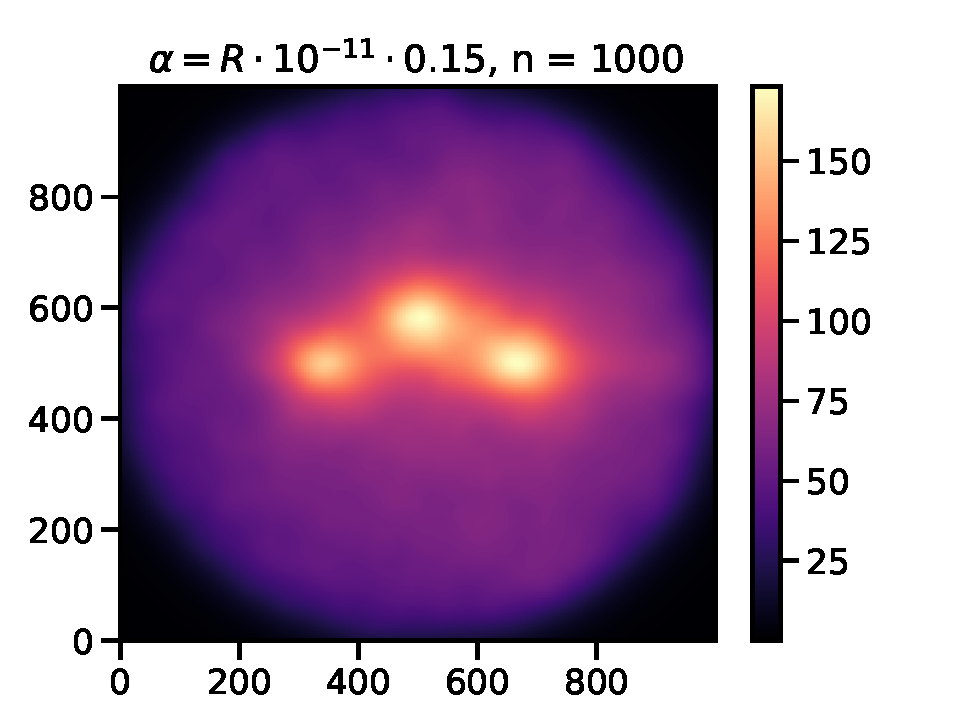
\includegraphics[width=.6\textwidth]{../img-mpi/graph1000-0.pdf}\hfill
    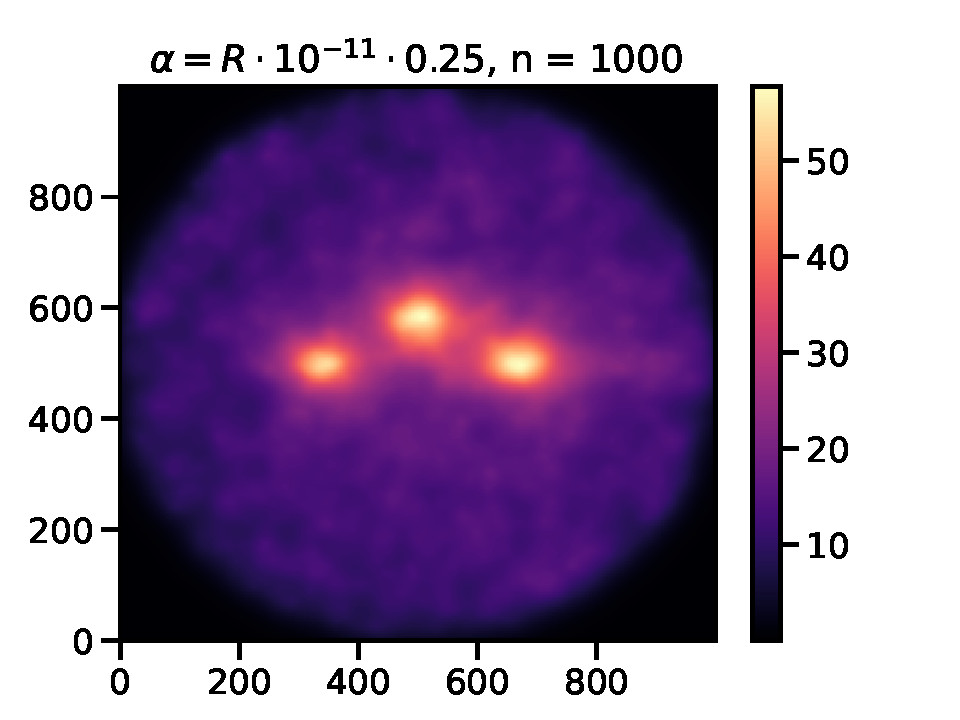
\includegraphics[width=.6\textwidth]{../img-mpi/graph1000-1.pdf}\hfill
    \\[\smallskipamount]
    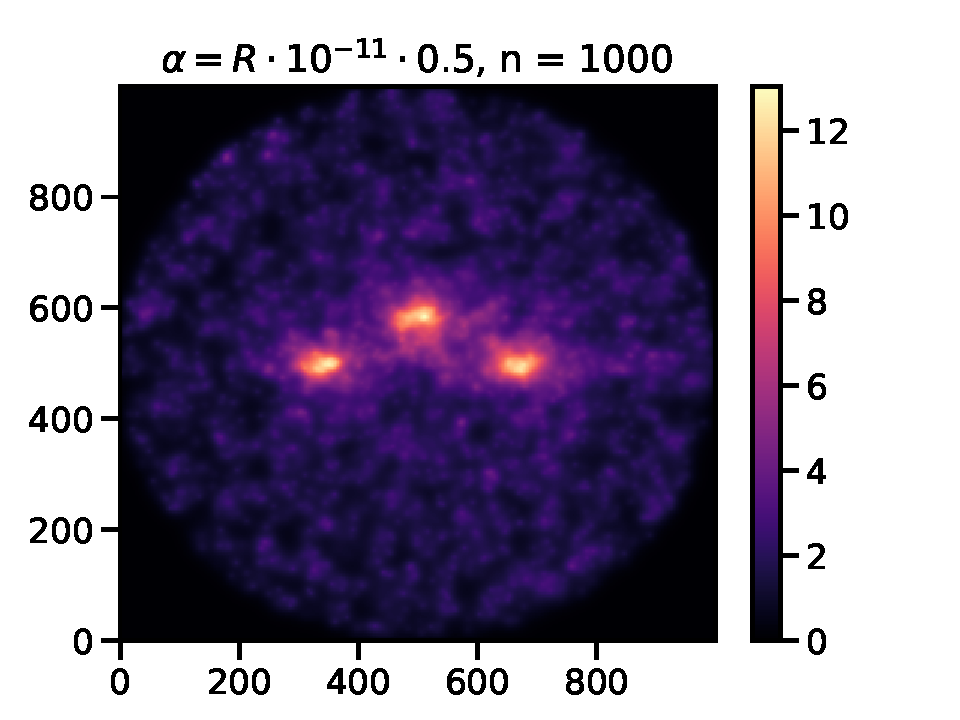
\includegraphics[width=.6\textwidth]{../img-mpi/graph1000-2.pdf}\hfill
    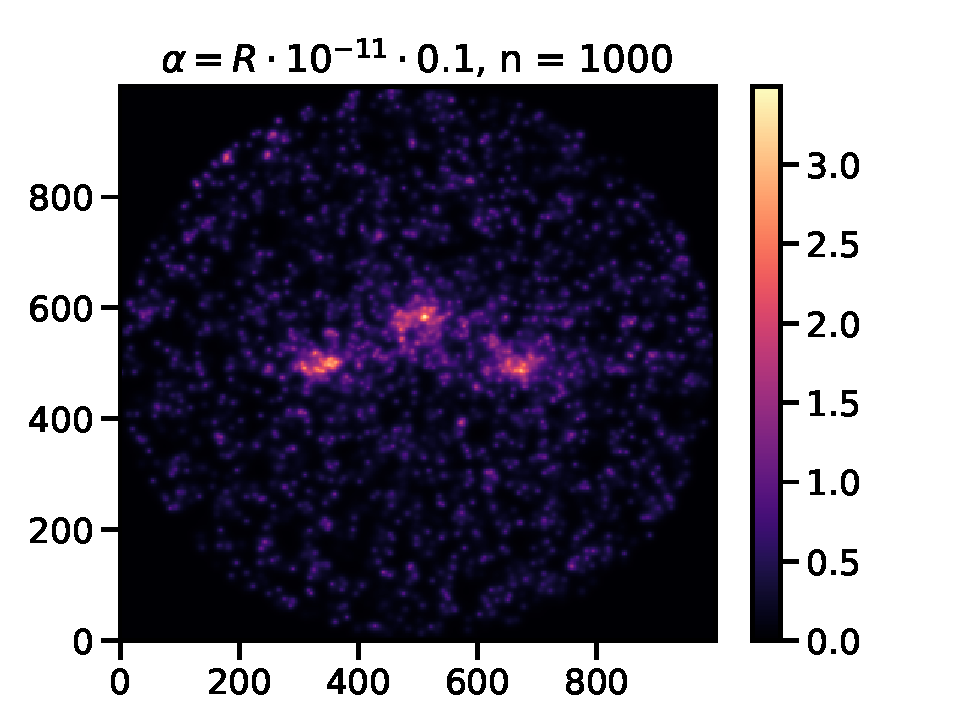
\includegraphics[width=.6\textwidth]{../img-mpi/graph1000-3.pdf}
    \caption{Comparison of the effect of the parameter \(\alpha\)
    for \(n_x = n_z = 1000\).}
\end{figure}

\section{MPI Implementation}

\subsection{Code}

Inside main:

\begin{verbatim}
    for (int k = 0; k < 8; k++) {
        // Size of total grid
        int n = n_arr[k];

        // Size of partial grid for each proccess
        int pn = n / size;

        if (n % size != 0)
            pn++;

        double *grid, *partial_grid;

        grid  = new double [pn * size * n];
        partial_grid  = new double [pn * n];

        for (int p = 0; p < 4; p++) {
            double alpha = alpha_arr[p];

            gettimeofday(&t1, 0);
            get_grid(grid, partial_grid, data, pn, n, alpha);
            gettimeofday(&t2, 0);
            
            if (rank == 0) {
                time = (1.0e6 * (t2.tv_sec - t1.tv_sec) +
                        t2.tv_usec - t1.tv_usec) / 1000.0;
                cout << n << " " << time << endl;
                print_output(grid, n, p);
            }
        }

        delete [] grid;
        delete [] partial_grid;
    }
    
\end{verbatim}

Function 'get\_grid':

\begin{verbatim}
    void get_grid(double *grid, double *partial_grid, double *data,
        int pn, int n, double alpha) {
        int rank;
        MPI_Comm_rank(MPI_COMM_WORLD, &rank);
        
        for (int i = 0; i < pn; i++)
            for (int j = 0; j < n; j++)
                partial_grid[i * n + j] = 0;

        for (int i = 0; i < pn; i++) {
            for (int j = 0; j < n; j++) {
                double xij = get_coord((double)(i + rank * pn),
                        (double)n);
                double zij = get_coord((double)j, (double)n);

                for (int k = 0; k < N; k++) {
                    double x       = data[k * 4 + 0];
                    double y       = data[k * 4 + 1];
                    double z       = data[k * 4 + 2];
                    double density = data[k * 4 + 3];

                    partial_grid[i * n + j] += density * exp(-alpha *
                            sqrt((x - xij) * (x - xij) +
                                 (z - zij) * (z - zij) +
                                 (y - 0)   * (y - 0)));

                }
            }
        }
        MPI_Gather(partial_grid, pn * n, MPI_DOUBLE, grid, pn * n,
                MPI_DOUBLE, 0, MPI_COMM_WORLD);
    }
\end{verbatim}

\subsection{Time Analysis}

\[
    T_{paral}(P, N) = T_{arithm}(N, P) + T_{comm}(N, P)
\] 

\[
    T_{arithm}(N, P) =
     N \cdot \frac{N}{P} \cdot M \cdot
 \underbrace{\tau \cdot T}_{\text{cost of arighmetic operations inside loop}}
\] 

\(M = 65536\) --- number of particles in input data.

\(T\) --- number of arithmetic operations.

\(\tau\) --- time for 1 arithmetic operation.

\[
    T_{comm}(N, P) = \left( \alpha + \frac{1}{\beta}
        \underbrace{\frac{N^2}{P}}_{\text{message length}}
            \right) 
            \underbrace{\sqrt{p} }_{\text{torus}}
\] 

\[
    S(N, P) = \frac{T_{arithm}(N, P)}{T_{paral}(N, P)}
\] 

\[
    E(N, P) = \frac{S(N, P)}{P}
\] 

\begin{table}[H]
    \centering
    \caption{Constants found through fitting.}
    \begin{tabular}{| c | c | c |}
        \hline
        Meaning & Notation & Value\\
        \hline
        Execution time of arithmetic operations within loop &
        \(\tau \cdot T\) &
        \( 2.32 \cdot 10^{-9}\) \\ % \pm 1.59 \cdot 10^{-3}\) \\
        Latency & \(\alpha\) &
        \(1.18 \cdot 10^{-4}\) \\ % \pm 8.11 \cdot 10^{1}\) \\
        Bandwidth & \(\beta\) &
        \(2.06 \cdot 10^{5}\) \\ % \pm 1.41 \cdot 10^{11}\) \\


        \hline
    \end{tabular}
\end{table}

\subsection{Speedup and Efficiency}

\begin{figure}[H]
    \centering
    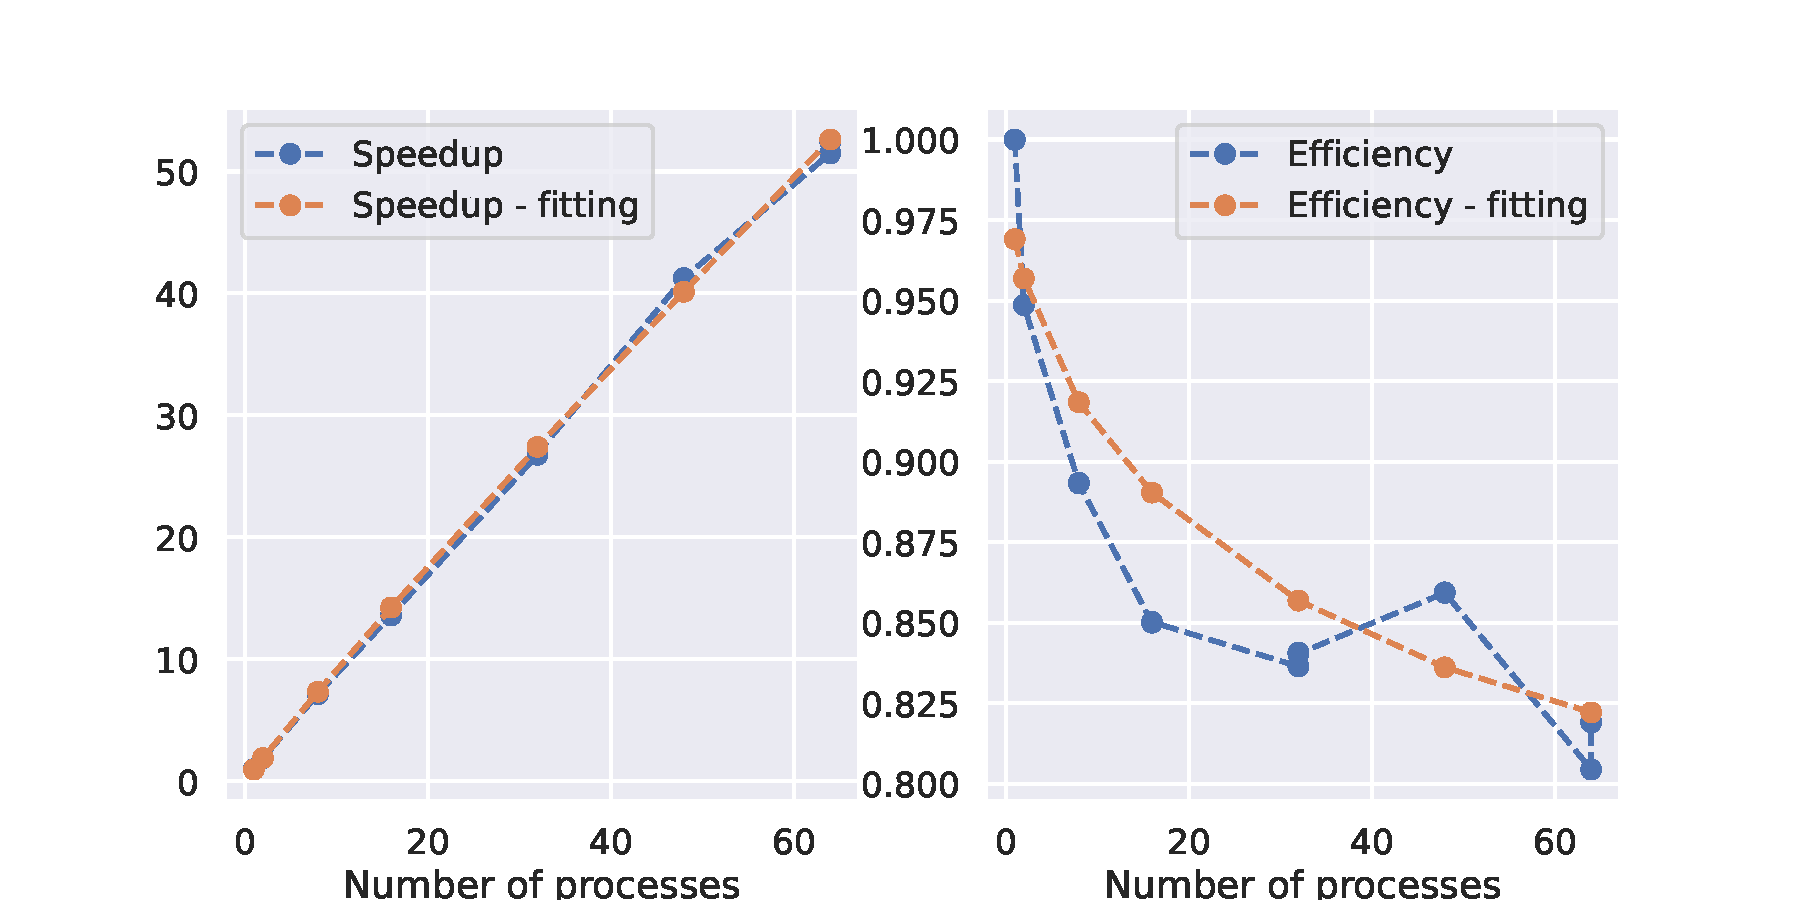
\includegraphics[width=\textwidth]{../img/speedup-mpi.pdf}
    \caption{Speedup and efficiency of the MPI implementation}
\end{figure}

\section{OpenACC Implementation}

\subsection{Code}

\begin{verbatim}
    #pragma acc data copyin(data[0:N*4]) copyout(grid[0:n*n])
    {
        #pragma acc parallel loop
        for (int i = 0; i < n; i++) {
            #pragma acc loop
            for (int j = 0; j < n; j++) {
                double xij = -R + (double)i / (double)(n - 1) * 2 * R;
                double zij = -R + (double)j / (double)(n - 1) * 2 * R;

                double cell_ij = 0;

                #pragma acc loop reduction(+:cell_ij)
                for (int k = 0; k < N; k++) {
                    double x       = data[k * 4 + 0];
                    double y       = data[k * 4 + 1];
                    double z       = data[k * 4 + 2];
                    double density = data[k * 4 + 3];
                    cell_ij += density * exp(-alpha *
                            sqrt((x - xij) * (x - xij) +
                                 (z - zij) * (z - zij) +
                                 (y - 0)   * (y - 0)));
                }
                grid[i * n + j] = cell_ij;
            }
        }
    }
\end{verbatim}

\subsection{Compiling: Unified Memory}

\begin{figure}[H]
    \centering
    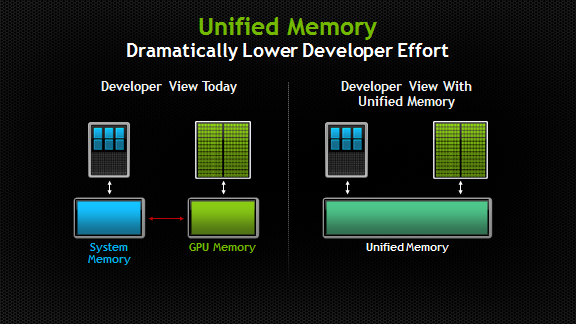
\includegraphics[width=0.8\textwidth]{img/unified-memory.png}
\end{figure}

\begin{verbatim}
pgc++ -lstdc++ -O2 -Wall -std=c++11 -acc -ta=nvidia:managed -Minfo=accel
\end{verbatim}

The 'managed' option lets us use Unified Memory.

Unified Memory creates a pool of managed memory that is shared between the CPU and GPU, bridging the CPU-GPU divide. Managed memory is accessible to both the CPU and GPU using a single pointer. The key is that the system automatically migrates data allocated in Unified Memory between host and device so that it looks like CPU memory to code running on the CPU, and like GPU memory to code running on the GPU.

\section{Time Metrics and Comparison
between MPI and OpenACC Implementations}

\begin{table}[H]
    \centering
    \caption{Time Comparison in ms}
    \label{tab:label}
    \begin{tabular}{| c | c | c | c | c |}
        \hline
        n    & CPU Sequential & GPU - OpenACC Unified Memory & GPU - OpenACC \\
        \hline \hline
10 & 28.32 $\pm$ 4.99 & 6.01 $\pm$ 0.33 & 132.39 $\pm$ 15.76 \\ \hline
20 & 42.46 $\pm$ 0.17 & 21.67 $\pm$ 0.02 & 140.18 $\pm$ 14.40 \\ \hline
50 & 201.92 $\pm$ 0.75 & 133.44 $\pm$ 0.56 & 186.12 $\pm$ 2.37 \\ \hline
100 & 604.44 $\pm$ 7.37 & 530.51 $\pm$ 0.54 & 261.90 $\pm$ 10.90 \\ \hline
250 & 2975.23 $\pm$ 0.19 & 3340.00 $\pm$ 12.82 & 1012.77 $\pm$ 18.90 \\ \hline
500 & 10938.35 $\pm$ 28.79 & 13524.73 $\pm$ 15.61 & 3655.64 $\pm$ 86.08 \\ \hline
750 & 23834.98 $\pm$ 35.10 & 30457.03 $\pm$ 13.72 & 8085.92 $\pm$ 145.40 \\ \hline
1000 & 41643.85 $\pm$ 1.59 & 54320.40 $\pm$ 19.08 & 13032.73 $\pm$ 70.97 \\ \hline
    \end{tabular}
\end{table}

\begin{figure}[H]
    \centering
    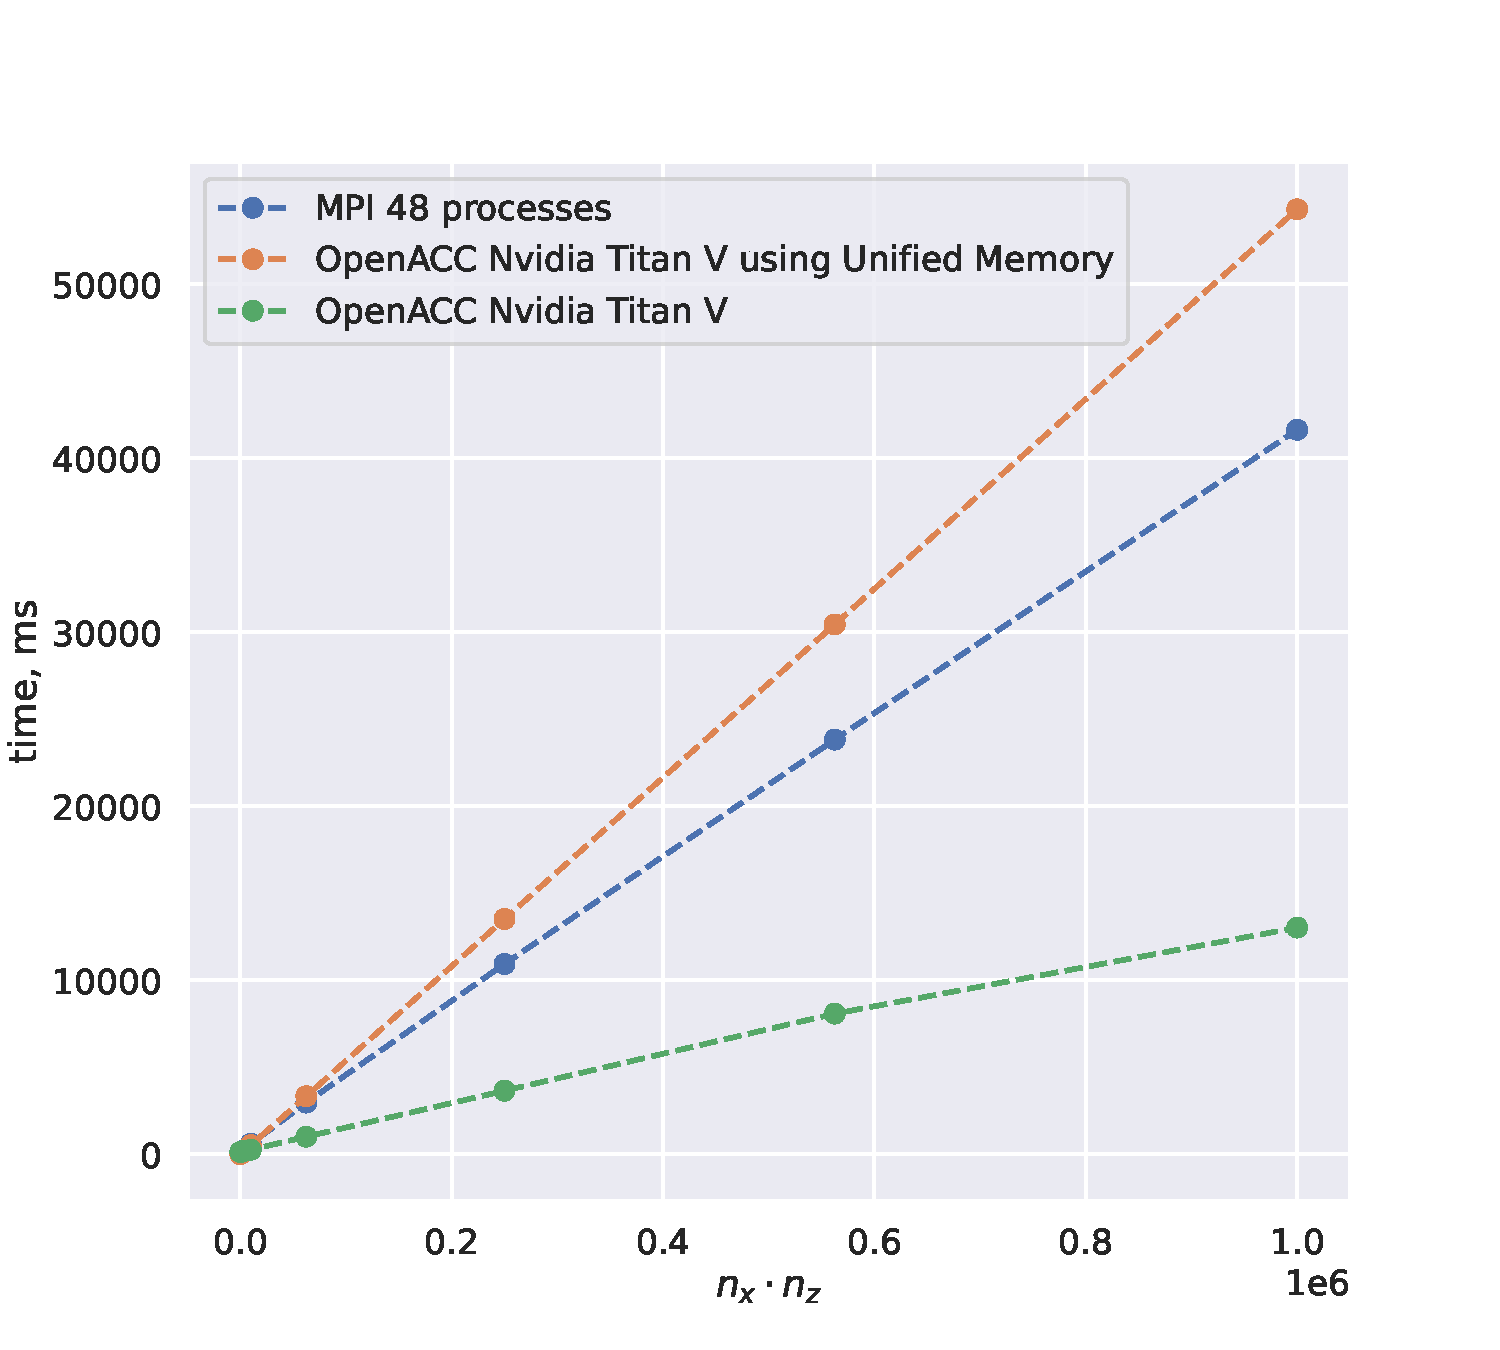
\includegraphics[width=\textwidth]{../img/time.pdf}
    \caption{Dependence of the run time at maximum
    optimization for different values of $n_x \cdot n_z$
    for MPI and OpenACC implementation.}
\end{figure}

\begin{figure}[H]
    \centering
    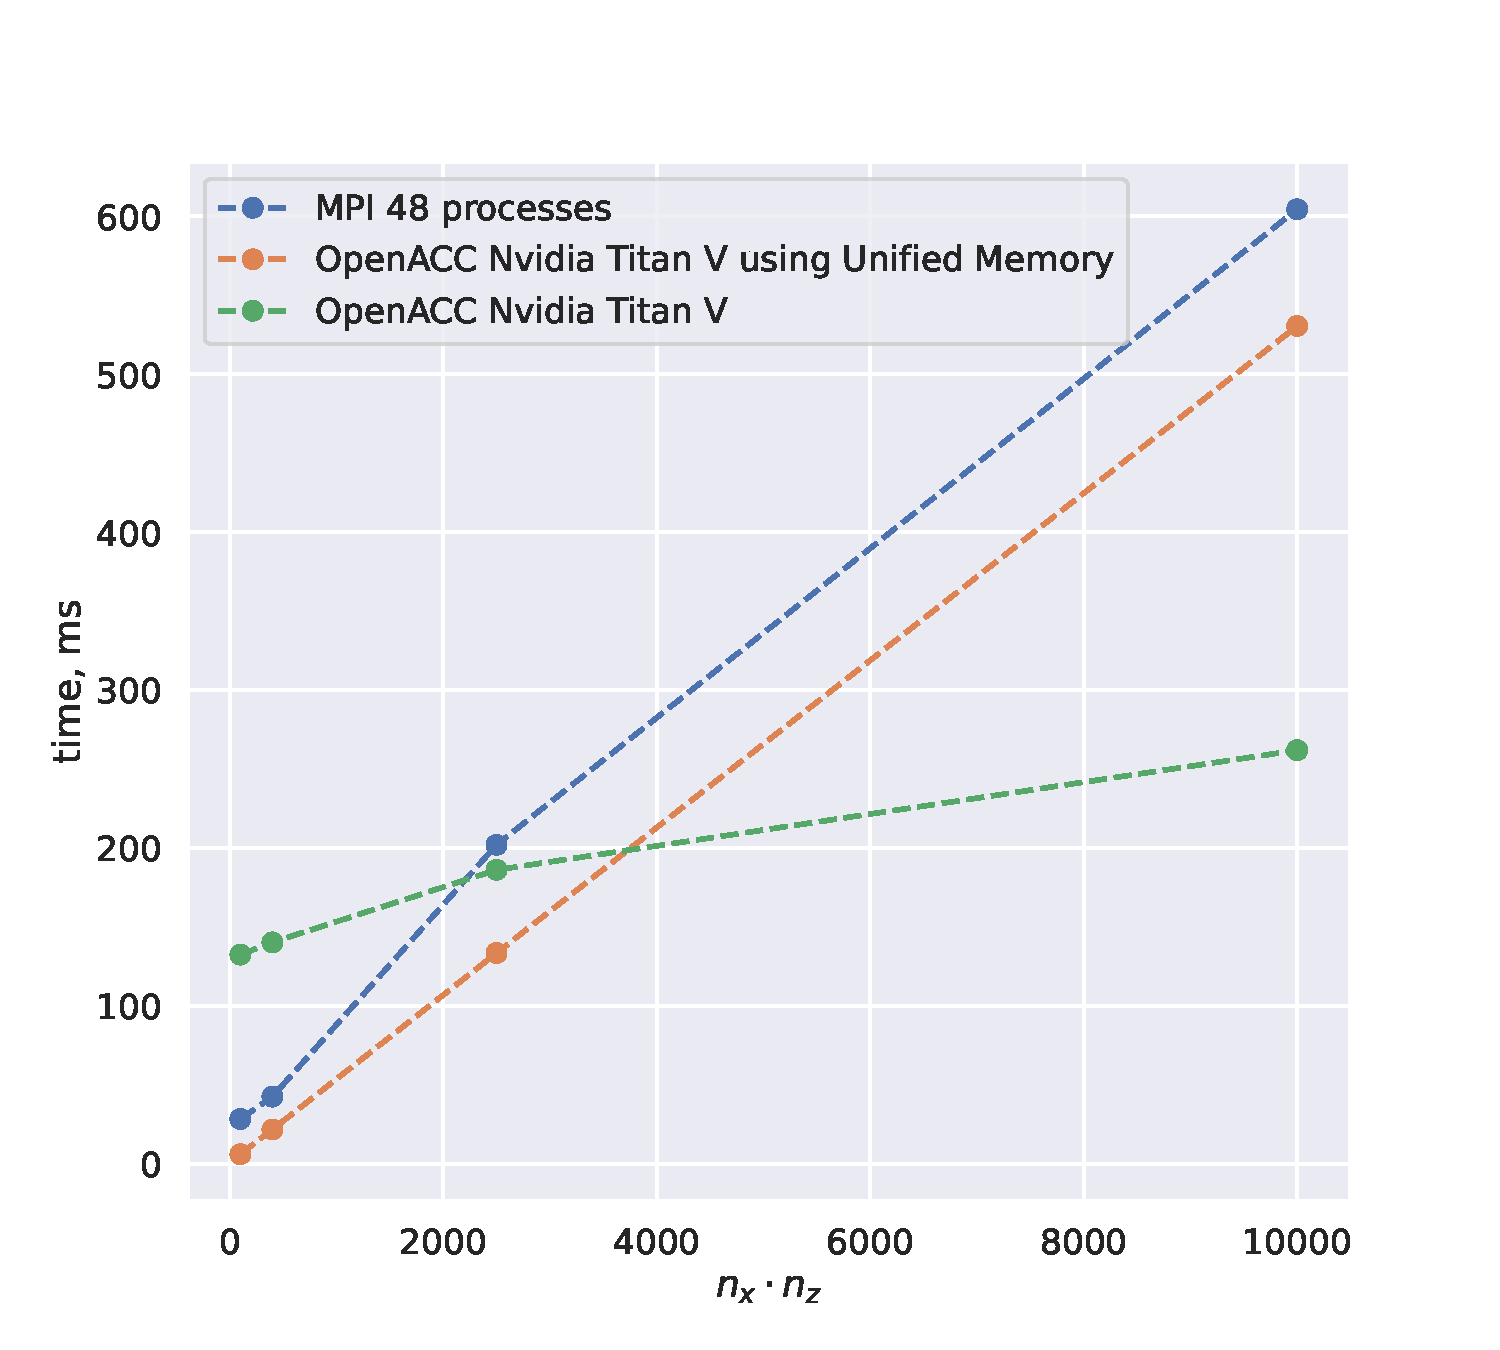
\includegraphics[width=\textwidth]{../img/time-small.pdf}
    \caption{Dependence of the run time at maximum
    optimization for small values of $n_x \cdot n_z$
    for MPI and OpenACC implementation.}
\end{figure}
    
\end{document}
